\chapter*{Proposition 12}
\label{prop:12}

\begin{figure*}[ht]
    \begin{center}
    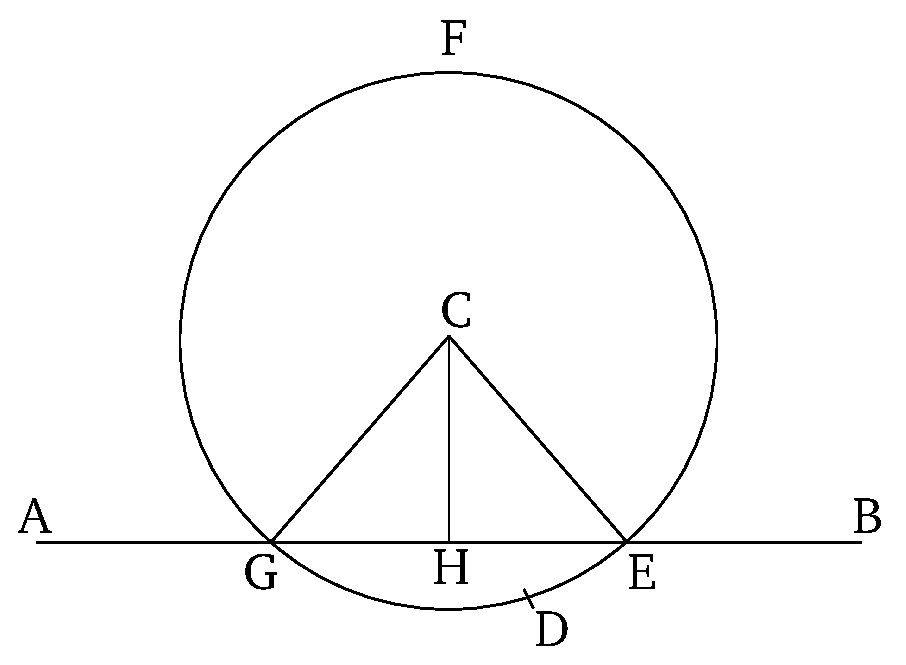
\includegraphics[width=0.5\linewidth]{figures/fig12e.eps}
    \label{fig:prop_12}
    \end{center}
\end{figure*}

To draw a straight-line perpendicular to a given infinite straight-line from a given point which is not
on it.\\

Let $AB$ be the given infinite straight-line  and $C$ the given point, which is not
on ($AB$). So it is required to draw a  straight-line  perpendicular to the
given infinite straight-line $AB$ from the given point $C$, which is not on
($AB$).

For let point $D$ have been taken at random on the other side (to $C$) of 
the straight-line $AB$, and let the circle $EFG$ have been drawn
with center $C$ and radius $CD$ [Post.~\ref{post:3}], and let the straight-line $EG$ have been cut
in half at (point) $H$ [Prop.~1.10], and let the straight-lines $CG$, $CH$,
and $CE$ have been joined. I say that the  (straight-line) $CH$ has
been drawn  perpendicular to the given infinite straight-line
$AB$ from the given point $C$, which is not on ($AB$).

For since $GH$ is equal to $HE$, and $HC$ (is) common, the two (straight-lines) $GH$, 
$HC$
are equal to the two (straight-lines) $EH$, $HC$, respectively, and the base $CG$ is
equal to the base $CE$. Thus, the angle $CHG$ is equal to the
angle $EHC$ [Prop.~1.8], and they are adjacent. But when a straight-line
stood on a(nother) straight-line makes the adjacent angles equal to one another, each of the equal angles is a right-angle, and the former straight-line is called a perpendicular to that upon which it stands [Def.~\ref{def:10}].

Thus, the (straight-line) $CH$ has been drawn perpendicular to the given infinite straight-line $AB$ from the given point $C$, which is not
on  ($AB$). (Which is) the very thing it was required to do.


\section*{Commentary}

\begin{proposition}\label{proposition_12}\lean{Elements.Book1.proposition_12}\leanok
    $A$ and $B$ are two distinct points on a line $AB$. $C$ is a point not on $AB$. Then, there must exist a point $H$ on $AB$ s.t., $\angle~AHC$ or $\angle~BHC$ is a right angle.
\end{proposition}
\begin{proof}
    \uses{proposition_8,proposition_10}\leanok
    See the original proof by Euclid.
\end{proof}
